\documentclass[a4paper, oneside, 12pt]{article}

% Paquets pour le Français
\usepackage[utf8]{inputenc} % Gestion encodages
\usepackage[T1]{fontenc} % ???
\usepackage[francais]{babel} % Typographie française

\usepackage{graphicx}
\usepackage{here}

\usepackage{lmodern}

\usepackage[top=2.5cm, bottom=3.5cm, left=2.5cm, right=2.5cm, footskip=2cm]{geometry}
\parskip=4pt

\newcommand\sectionSpeciale[1]{\addcontentsline{toc}{section}{#1}\section*{#1}}

\def\www{\emph{W3+}}
\def\siemens{\emph{Siemens}}

\author{ Lucien \sc{Guimier} (F5, \siemens) \\ Timothée \sc{Hamon} (F3, \www) }
\title{Dossier management}

\begin{document}

\maketitle

\begin{center}
\vfill
\vfill

\includegraphics[height=1.5cm]{img/logo-siemens.png}
\vfill

\includegraphics[height=2.3cm]{img/logo-www.png}
\vfill
\end{center}

\thispagestyle{empty}

\newpage
\setcounter{page}{1}
\sectionSpeciale{Introduction}

Ce dossier a pour but de présenter les différences et les similitudes entre les deux entreprises que sont \siemens\ et \www. \siemens\ est une multinationale allemande où Lucien {\sc Guimier} a effectué son stage, alors que \www\ est une petite ESN (entreprise de services du numérique) située au nord de Vichy.

\vfill

\tableofcontents

\vfill

\newpage
\section{Organisation des entreprises}

\subsection{\siemens}

\siemens\ est un groupe employant actuellement environ $348~000~$employés et dont la structure a connu de nombreuses variations depuis sa création, notamment ces dernières années. Il est actuellement dirigé par Joe {\sc Kaeser} et structuré autour de cinq grands pôles :

\begin{enumerate}
	\item \textit{Energy} ;
	\item \textit{Healthcare} ;
	\item \textit{Infrastructure \& cities} ;
	\item \textit{Industry} ;
	\item autres.
\end{enumerate}

Lucien {\sc Guimier} a effectué son stage dans la branche \textit{Industry}, plus particulièrement dans le le département \textit{Factory Automation}, qui développe un logiciel de configuration du matériel d’automatisation. La taille de ce logiciel nécessite plusieurs centaines de développeurs répartis sur plusieurs sites, en Allemagne et à l’étranger. Il a travaillé sur un important site de \siemens\ regroupant des équipes de plusieurs branches du groupe.

\subsection{\www}

\www\ est une petite entreprise comptant actuellement 12 employés, issue de la séparation de \emph {CS3I} en 2008. Son domaine d'activité est essentiellement centré sur l'infogérance et cette petite ESN a la particularité d'avoir un client principal qui occupe plus de 70$~$\% de son activité. Les deux stagiaires étaient affectés au pôle développement de \www.

\ 

\begin{figure}[H]
	\centering
	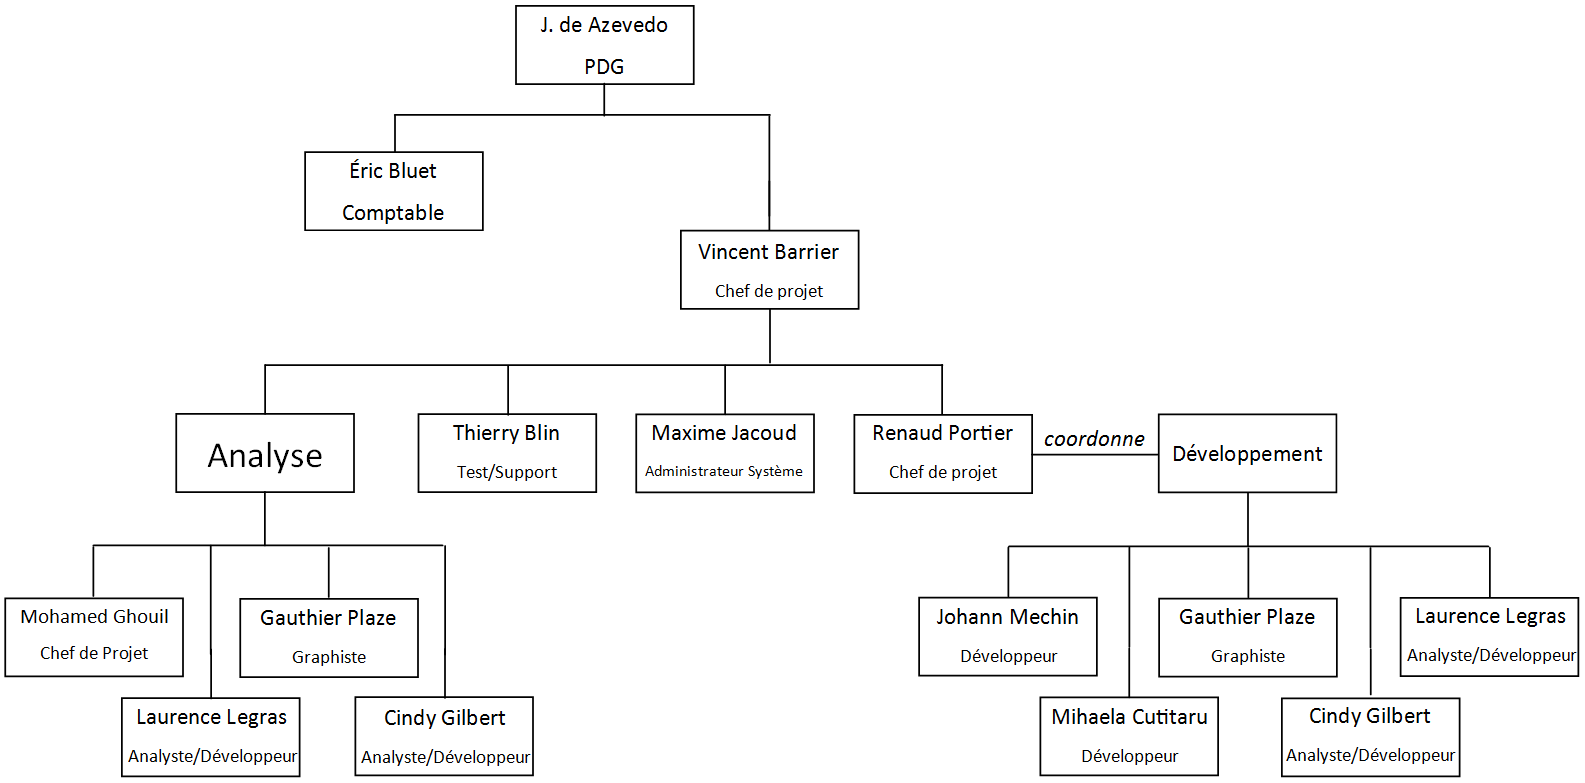
\includegraphics[width=16cm]{img/org-www.png}
	\caption{Organigramme de \www}
\end{figure}

\newpage
\section{Organisation des équipes}

\subsection{Organisation du travail}

\subsubsection{Organisation à court terme}

À \www, le travail est organisée selon la méthodologie \emph{Scrum} : les différents projets sont découpés en tâches courtes (une à huit heures) réparties sur une période de deux à quatre semaines. À la fin d’une telle période, le produit est en principe déployé chez le client. Chaque matin, l’équipe se réunit pour discuter de l’avancement des tâches et des éventuels problèmes rencontrés.

\begin{figure}[H]
	\centering
	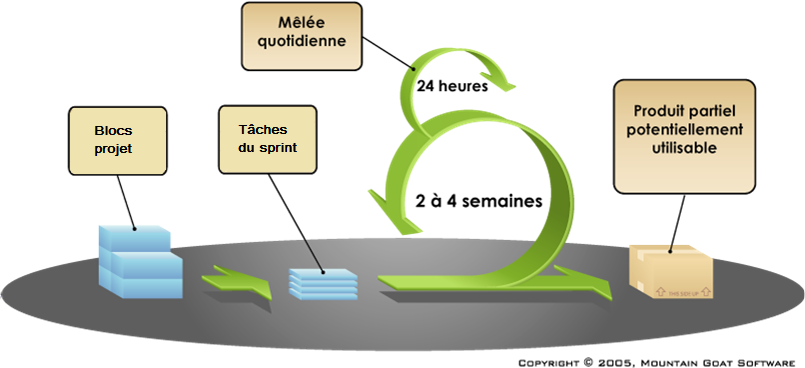
\includegraphics[width=12cm]{img/scrum.png}
	\caption{Schéma de la méthodologie \emph{Scrum}}
\end{figure}

La résolution des tâches et l’association de celle-ci avec les modifications du code est suivies grâce à TFS (\emph{Team Foundation Server}).

Une réunion supplémentaire de 11$~$h à 12$~$h le lundi permet aux développeurs de partager les problèmes rencontrés et les solutions qu’ils y ont apportées. C’est aussi l’occasion pour le chef développeur de signaler les défauts globaux du développement.

\ 

La partie de l’équipe de \siemens\ où était intégrée Lucien {\sc Guimier} se réunit deux fois par semaine, le lundi et le mercredi, pour discuter de l’avancement des tâches. Le suivi de celles-ci est réalisé grâce à un tableau \emph{Kanban} (autre méthodologie associée à \emph{Agile}) : les tâches sont représentées par des cartons avec leur description, disposés dans des colonnes selon leur avancement (à faire, en cours, fini).

Un écran permet d’avoir un aperçu de l’avancement de la correction des problèmes et d’être informé des prochains jalons.

\ 

Les deux méthodologies sont assez similaires ; seule la fréquence de déploiement chez le client change : le logiciel est déployé chez \www\ au minimum une fois par mois, tandis que l’équipe de \siemens\ travaille sur la prochaine version majeure du logiciel développé, intégrant uniquement leurs modification à la version commune, la version majeure étant publiée moins d’une fois par an.

\newpage

\subsubsection{Organisation à long terme}

Tous les mois, l’équipe de \siemens\ (entière) organise un petit déjeuner de projet (« \textit{Projektfrühstück} »), durant lequel un ou deux membres de l’équipe présentent les nouveautés. Les présentations sont suivies en consommant un assortiment de jus, gâteaux, fromages, pains et charcuterie ; la consommation commence un peu avant, laissant le temps pour des discussions libres.

\subsubsection{Séminaires et formations}

Aucun séminaire ne semble organisé à \www, tandis qu’un moins un a eu lieu sur le complexe de \siemens\ pendant la période du stage.

\www\ fournit des formations à ses employés sur demande, à condition que celle-ci soit en concordance avec son domaine de travail et ses besoins. Elles sont en général réalisées par groupes.

% TODO
Nous n’avons pas d’informations sur les formations dispensées à \siemens.

\vfill

\subsection{Interactions entre collègues}

\subsubsection{Pauses pendant les horaires de travail}

Dans les deux entreprises, un espace est réservé pour les pauses café, chacun équipé d’une machine à café. Malgré les recommandations, l’équipe de \siemens\ dispose de plus d’une cafetière directement sur une table disposée entre les bureaux.

\ 

À \www, toute l’équipe est attendue à la pause du matin, vers 9$~$h —$~$avant la réunion journalière$~$— et une seconde pause est possible vers 14$~$h. Il arrive qu’un employé —$~$parfois plusieurs$~$— apportent des viennoiseries ou des gâteaux pour toute l’équipe en guise de petit déjeuner. Ces petits déjeuners ont en particulier lieu lors d’un anniversaire ou après un déploiement.

\ 

Du fait de la présence d’une cafetière au centre des postes de travail, l’équipe de \siemens\ n’a pas de telles pauses fixes, les cafés étant consommés directement pendant le travail. Les autres équipes cependant, semblent avoir des pauses communes à la salle café.

À plusieurs reprises, des goûters ou des petit déjeuners ont été organisés par certains employés à l’occasion d’événements particuliers comme un départ en voyage de noces ou des anniversaires.

\vfill

\newpage

\subsubsection{Pauses déjeuner}

\www\ ne disposant pas de cantine, les employés peuvent manger dans la salle de repos, équipée pour réchauffer des plats. Environ les deux tiers de ceux-ci l’utilisent quotidiennement. Environ une fois par mois, un repas collectif est organisé par les employés.

\ 

Le complexe de \siemens\ inclut deux cantines où les membres de l’équipe se rendent par groupes de quatre à huit personnes en général.

\ 

Dans les deux équipes, la pause dure environ une heure et les sujets de conversation concernent rarement le travail en cours.

\subsubsection{Rencontres hors travail}

Timothée {\sc Hamon} a participé à une pendaison de crémaillère chez un de ses collègues. À \siemens, conformément à l’habitude allemande, aucune rencontre au domicile d’un employé n’a eu lieu ; un repas a cependant été organisé à une brasserie proche et une randonnée avait lieu après le départ de Lucien {\sc Guimier}.

Sans y avoir participé, nous savons qu’un repas de Noël est organisé à \www\ et que d’autres équipes de \siemens\ organisent des balades en vélocipède.

\vfill

\section{Gestion du stagiaire}

\subsection{Arrivée sur le projet}

À \www, une réunion d’arrivée a permis de présenter l’entreprise aux deux stagiaires et de donner un rapide aperçu des deux sujets. Durant l’après-midi du premier jour, chaque stagiaire a eu un entretien de présentation plus avancée avec son tuteur, incluant notamment les objectifs et les outils du stage. Après le week-end, Timothée {\sc Hamon} a été immédiatement intégré dans l’équipe.

\ 

À \siemens, une réunion de sécurité était organisée la première journée et une première présentation des outils du stage a été réalisée par le tuteur de Lucien {\sc Guimier}. Deux réunions ont été organisées les jours suivants afin de préciser l’environnement du projet et les objectifs du stage, pendant que le stagiaire installait les outils nécessaires sur son poste de travail.

Au bout de quelques semaines, une réunion a été organisée avec tous les stagiaires pour présenter les sujets des uns aux autres et à leurs tuteurs.

\vfill

\newpage

\subsection{Gestion quotidienne}

Timothée {\sc Hamon} était partiellement intégré à son équipe : ses tâches liées à la maintenance de l’existant faisaient partie de la liste des tâches de l’équipe, tandis que son travail de recherche ne l’était pas. Durant ses phases de recherche, il avait une réunion hebdomadaire avec son tuteur pour faire le point sur son avancement et définir ses prochains objectifs.

\ 

Lucien {\sc Guimier} avait un projet séparé du reste de l’équipe, mais était intégré aux réunions bihebomadaires, où il devait indiquer son avancement et ses objectifs proches comme le reste de l’équipe. À quelques occasions, son tuteur est venu voir l’avancement réel du travail et proposer des évolutions.

\ 

L’intégration des stagiaires était donc assez similaire dans les deux entreprises, avec un suivi au minimum hebdomadaire de l’avancement.

\subsection{Fin de stage}

Au terme du stage, une réunion a été organisée à \www\ avec le tuteur du stagiaire et le chef développeur, afin d’établir les objectifs atteints, les actions restant à effectuer à court terme et les axes d’amélioration future.

\ 

À \siemens, une réunion avec tous les stagiaires a été organisée pour présenter le résultat des différents projets. Le dernier jour, le tuteur a effectué une évaluation de la qualité du travail du stagiaire et de son intégration dans l’équipe.

\vfill

\sectionSpeciale{Conclusion}

Comme il a été présenté tout au long de ce dossier, les deux entreprises —$~$bien que de tailles et de pays différents$~$— ont une façon similaire de diriger leurs employés. En effet, nous retrouvons une méthodologie de travail très proche, des lieux de rassemblement pour les repas et les pauses ainsi qu'un suivi régulier des employés dans leur travail. Là où \siemens\ se différencie de \www, c'est au niveau des déploiements pour ses clients. Du fait de sa relation très priviligiée qu'entretien \www\ avec son client principal, le déploiement des différentes améliorations est régulier. Alors que pour \siemens, du fait de leur nombre important de client, les mises à jour sont plus espacées.

\vfill

\end{document}
